\pdfbookmark{Introduction}{Introduction}
\chapter{Introduction}
\begin{quote} 
\it This chapter gives a basic introduction to  \ac{DSCs} and \ac{MPPT}.It also defines the Scope, Goals, Objective and the Research methodology for the thesis.
\end{quote}

\section{Background}

Our ever increasing reliance on electrical and electronic equipment intensified our search for new sources of energy. Dwindling fossil-fuel reserves are not something we can rely on in the long-term. Alternate energy sources must be efficient, cost-effective and ecologically friendly. The harnessing of solar energy becomes a very attractive proposition. A moderately efficient solar cell array (8\% - 10\% efficiency) covering a small portion of the earth's surface would be able to provide an enormous amount of electric power and thus reduce greenhouse-gas emissions \cite{kalyanasundaram2010dye}. However, the current high cost of solar panels made from traditional inorganic semiconductors imposes a restriction on their mass usage.
 **picture about the losses  Solar energy intercepting Earth [toivola2010dye]**
 
 \subsection{Dye-Sensitized Solar Cells(DSCs)}
  Photovoltaic devices are based on the concept of charge separation at an interface of two materials of different conduction mechanism. To this date, the field has been dominated by Solid-state junction devices, usually made of silicon, and profiting from the experience and material availability resulting from the semiconductor industry. The dominance of the photovoltaic field by inorganic Solid-state junction devices is now being challenged by the emergence of a third generation of cells, based on nano-crystalline oxide and conducting polymer films \cite{gratzel2004conversion}. Crystalline silicon being the first; and thin film technologies such as \ac{CdTe}, \ac{CIGS}, \ac{CIS} and \ac{a-Si} being examples of the second generation \cite{toivola2010dye}.\\
  
  Solar energy can be converted into electricity by a variety of technologies that can also be divided into four classes: Concentrator systems, wafer-based crystalline silicon, thin-film technologies and emerging technologies\cite{wenger2010strategies}.\\
  
    \begin{figure}[H]
    \begin{center}
    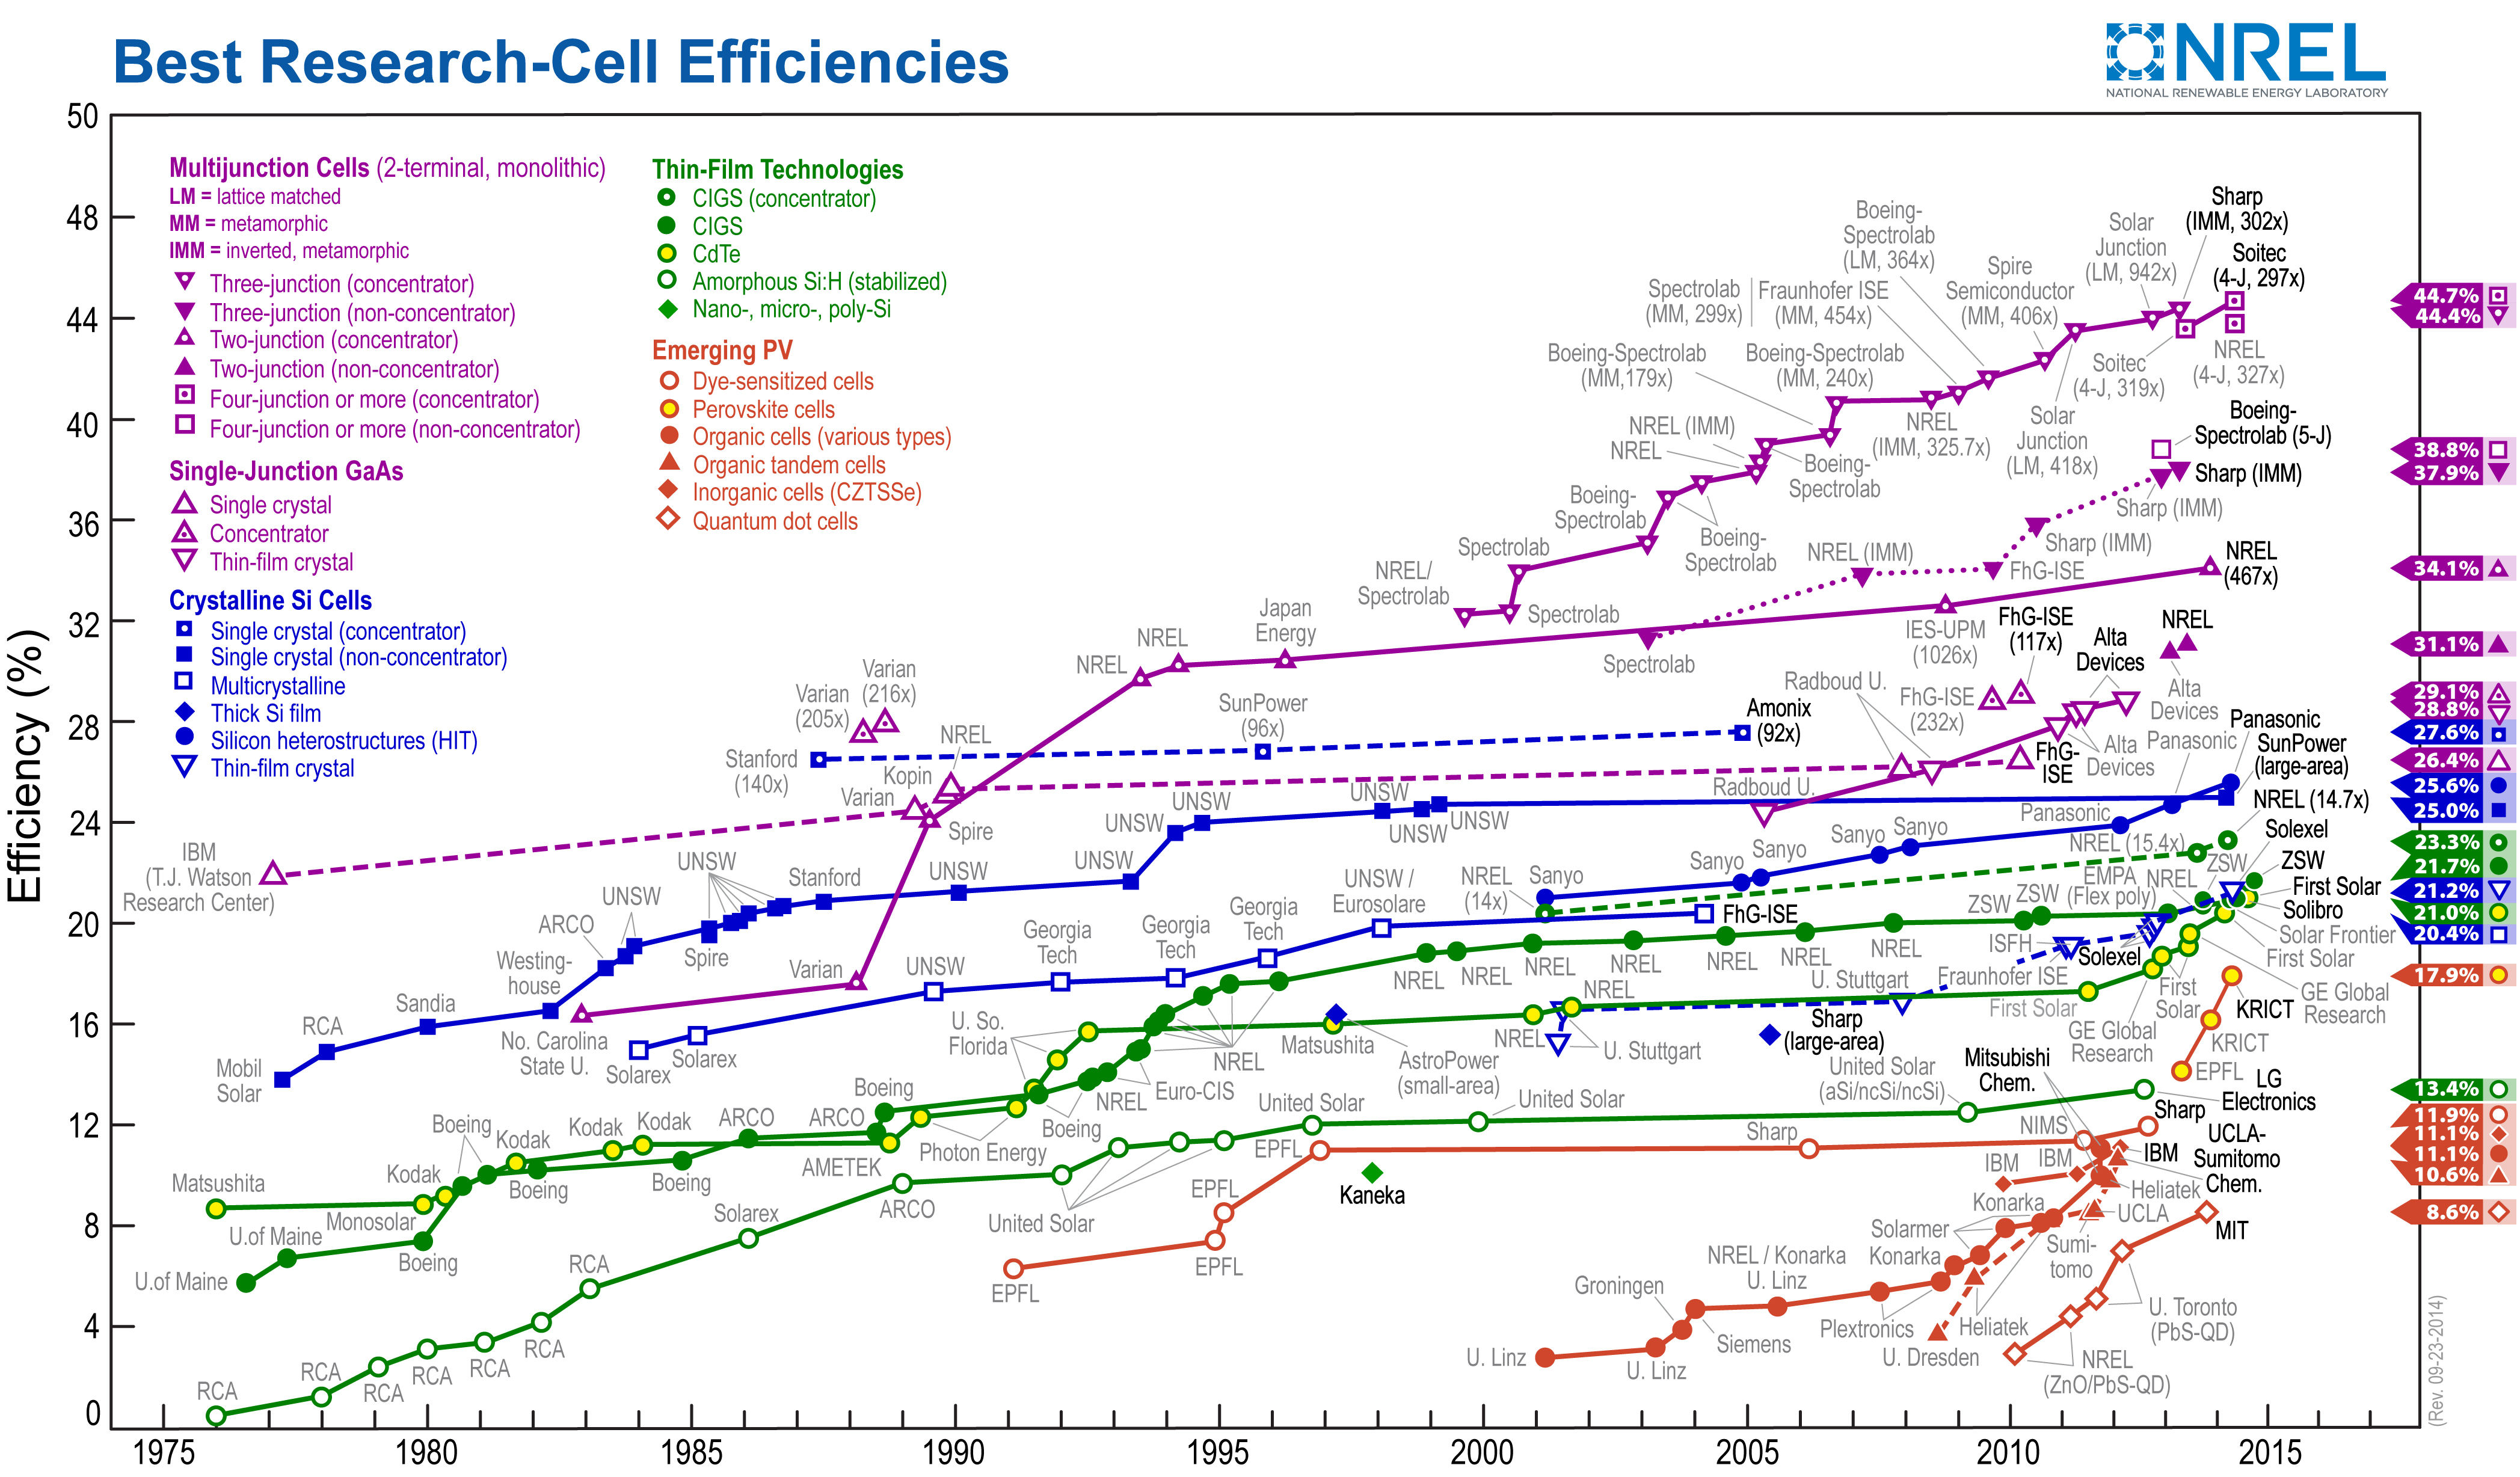
\includegraphics[width=\textwidth]{images/efficiency_chart.jpg}
    \caption{Research Cell Efficiency Records \cite{nrel_Research_Cell} }
    \label{fig:Cell_eficency}
    \end{center}
    \end{figure}
  
  Dye-sensitized solar cells(\ac{DSCs}) are the most promising of the third and latest generation of solar cells. Under development for the last 20 years, this technology is ready for large scale commercialization to provide robust, efficient and affordable solar energy to the masses. Unlike previous generation cells, \ac{DSCs} is a Photo-electro-chemical device whose principle of operation is similar to Photosynthesis seen in plants.\\

 \subsection{Advantages of DSCs }
  
  The rate of adoption for solar cells is slow. A major contributing factor for this is the predominant type of solar cells used today -ones made from silicon, which are quite expensive and are complex to manufacture. This has lead to intensive research into alternative solar cells in the past decade. \ac{DSCs} have many advantages over their 1st and 2nd generation counterparts. They offer transparency, low cost, and high power conversion efficiencies under cloudy and artificial light conditions.\ac{DSCs} work even in low-light conditions such as non-direct sunlight and cloudy skies.They are easy and economical to manufacture,with the major constituent materials available in abundance in most counties. This copious availability of raw material also enables us to scale the manufacturing to Tera-Watt levels with relative ease. Raw-materials are non-toxic and there are no noxious emissions during fabrication - leading to sustainable manufacturing. \\
  
   
  \begin{figure}[H]
  \begin{center}
  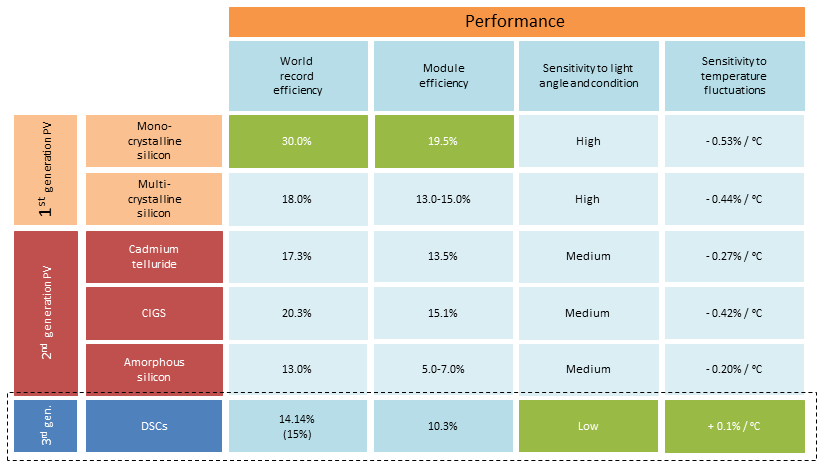
\includegraphics[width=\textwidth]{images/3rd_gen}
  \caption{ Three generations of cells –  Performance}
  \label{fig:3rd_gen}
  \end{center}
  \end{figure}
 
  **Add more details about Advantage of DSC over conventional cells **\\
 
   
\section{Maximum Power Point Tracking(MPPT)}

A Photo-Voltaic (PV) array that functions under uniform radiation and temperature conditions presents an I–V and P–V characteristic as the one shown in Figure ~\ref{fig:IVgraph} and Figure ~\ref{fig:PVgraph},respectively. As can be observed, there is a single point, called \ac{MPP}, where the array provides the maximum power possible for these environmental conditions (radiation and temperature), and so functions with the maximum performance. When a load is connected directly to a PV array (direct coupling), the operation point is defined by the intersection of its I–V characteristics, as shown in Figure ~\ref{fig:IVgraph}. In general, this operation point does not coincide with the \ac{MPP}. Thus, in direct coupling systems, the array must be over-dimensioned to guarantee the power demand of the load. Obviously, this implies a more expensive system. To solve this problem, a DC/DC  converter with an algorithm for the automatic control of its duty cycle “${\delta}$” is inserted between the photovoltaic array and the load , resulting in what is known as \ac{MPPT} system. The MPPT must control the voltage or current (through the ${\delta}$ the converter) of the PV array regardless of the load, trying to place it in the \ac{MPP}.Therefore,the MPPT must find the optimal ${\delta}$ for the operation point of the PV array to coincide with the \ac{MPP}\cite{enrique2010reliable}.\\

Although the solution to operating in the \ac{MPP} may seem straightforward, it is not! This is because the location of the \ac{MPP} in the I–V curve of the PV array is not known beforehand. This point must be located, either by mathematical calculations over a valid model, or by using some search algorithm. This implies even more difficulty if we consider the fact that the \ac{MPP} presents non-linear dependencies with temperature and radiation\cite{enrique2010reliable}\\





  \begin{figure}[H]
  \begin{center}
  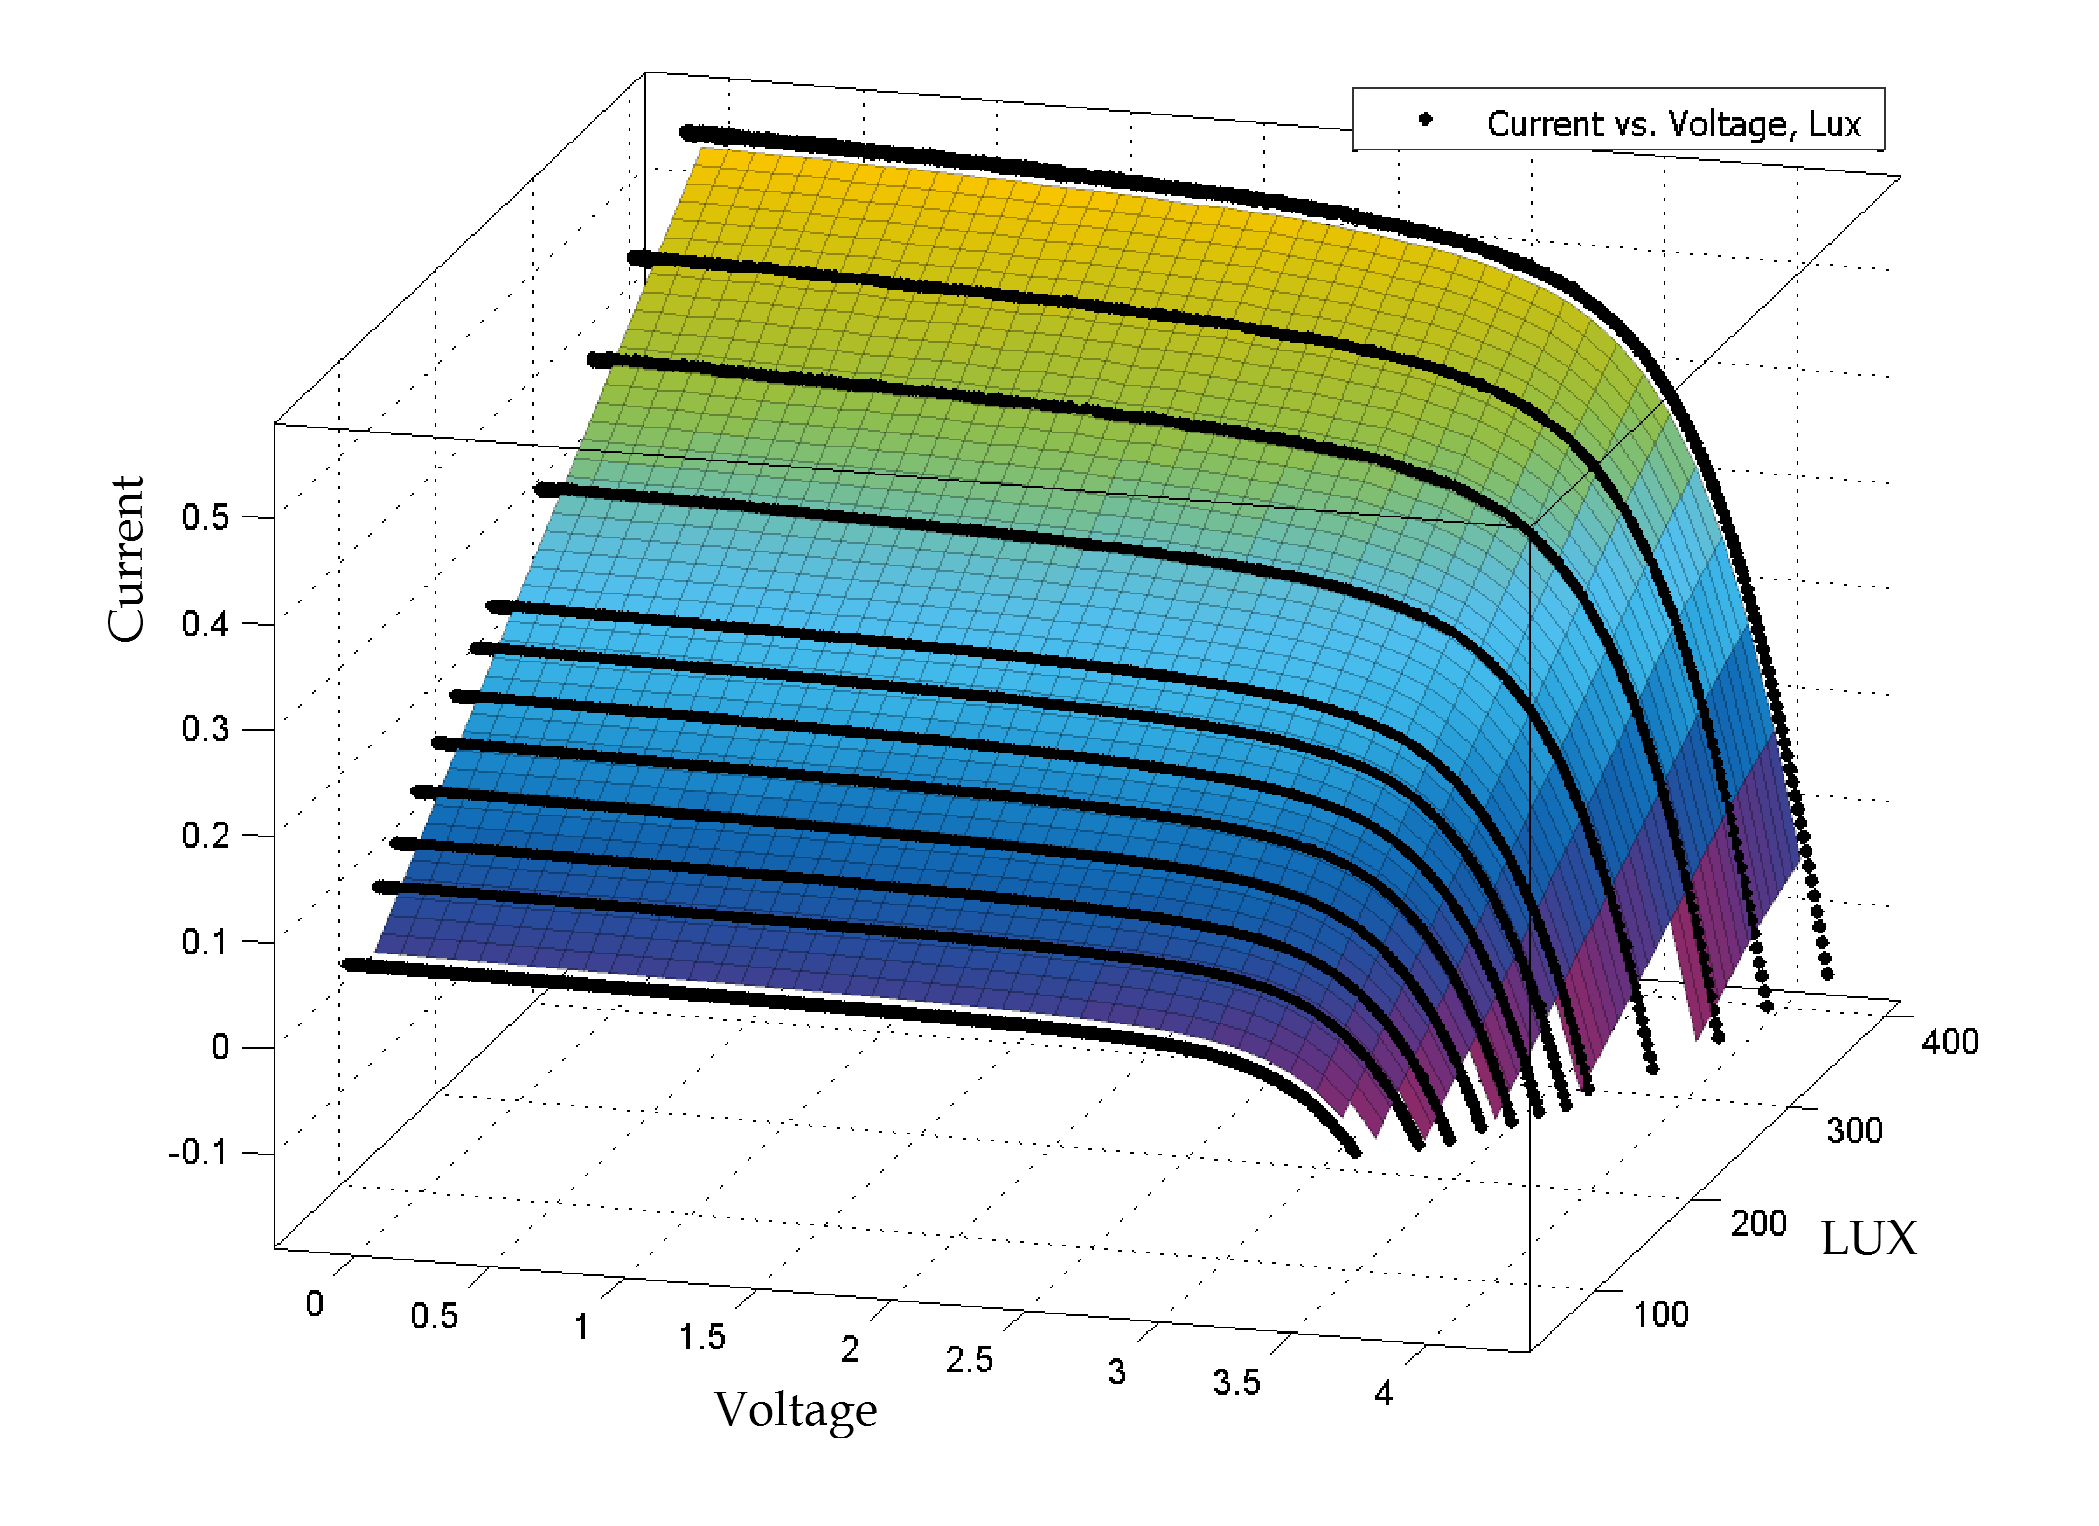
\includegraphics[width=\textwidth]{images/I-V-lux}
  \caption{I-V-Lux}
  \label{fig:IVgraph}
  \end{center}
  \end{figure}
  
    \begin{figure}[H]
    \begin{center}
    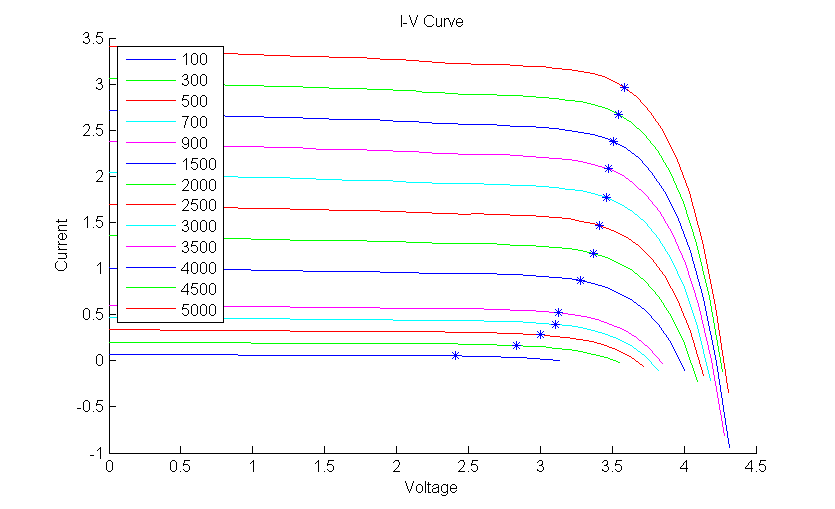
\includegraphics[width=\textwidth]{images/IV_lux_MPP}
    \caption{I-V Graph, MPPT marked with '*'}
    \label{fig:IV_mppgraph}
    \end{center}
    \end{figure}
  
  \begin{figure}[H]
  \begin{center}
  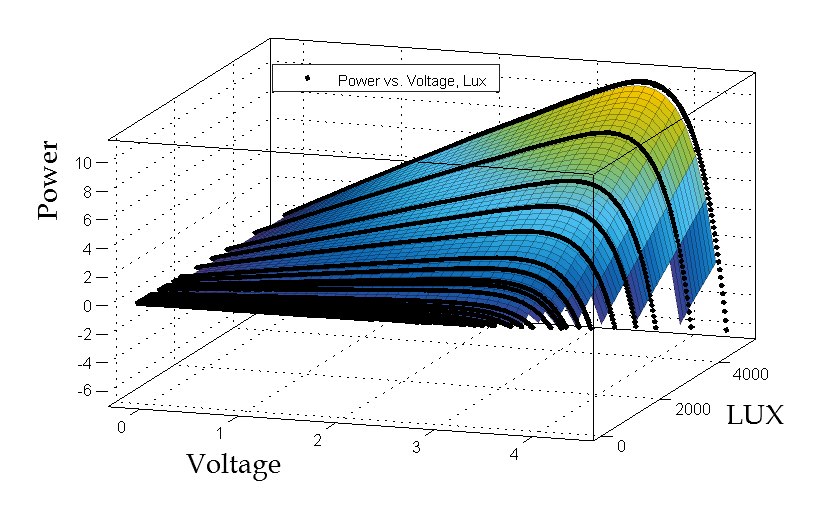
\includegraphics[width=\textwidth]{images/PV_LUX}
  \caption{ P-V Lux}
  \label{fig:PVgraph}
  \end{center}
  \end{figure}

As such, numerous \ac{MPPT} methods have been developed and implemented\cite{ngan2011study} \cite{esram2007comparison} \cite{eltawil2013mppt} . The methods vary in complexity, sensors required, convergence speed, cost, range of effectiveness, implementation hardware, popularity, and in other respects\cite{reza2013classification} \cite{dondi2008modeling}. They range from the almost obvious (but not necessarily ineffective) to the most creative (not necessarily most effective). In fact, so many methods have been developed that it has become difficult to adequately determine which method, newly proposed or existing, is most appropriate for a given PV system.Some of the most popular being: \\

  
\begin{itemize}
 \item Perturb and Observe Method
 \item Incremental Conductance Method
 \item Fractional Open Circuit Voltage Method
 \item Fixed duty cycle Method
 \item Pilot Cell Method
 \item Fractional short-circuit current Method
 \item Fuzzy-logic controller
\end {itemize}
 
 
 \section{Scope, Thesis goals and Objectives}

This thesis focuses on the finding a practical and usable \ac{MPPT} algorithm that is optimised to be used with current \ac{DSCs}.\\


The objectives of the thesis can be summarized as:
\begin{itemize}

\item Develop an electrical model for DSCs and verify the accuracy of said model.
 
\item Compare and optimise the following Maximum Power Point Tracking (MPPT) algorithms for compatibility with the above Model using MATLAB{\textregistered} and Simulink{\textregistered}.
	\begin{enumerate}
		\item \ac{PnO} Method.
		\item \ac{ICM}.
		\item \ac{FOCV} Method.
		
	\end{enumerate}
\item Setting up the test environment   
\item Execution of test cases on prototype developed, based on two of the best optimised algorithms, with recordable test results.
\item Develop reference designs for production.
\item Internal report.
\item  Master thesis report. 
\end {itemize}

\section{Thesis outline}
\begin{itemize}
\item Chapter 1 Presents the background and the main objectives of this thesis. \\
\item Chapter 2 Contains the prior research and literature that this thesis was based on. It also discusses the operating principles/state-of-the-art  of \ac{DSCs} and of \ac{MPPT}. \\
\item Chapter 3 Concerns the  research methods, measurement techniques and implementation of the thesis.
\item Chapter 4 Gives a summary of the results. 
\item The thesis is concluded and future work talked about in Chapter 5.
\end {itemize}

\section{Research methodology}
The implementation of the thesis is the four steps. 
\begin{itemize}
\item Develop a suitable model for the \ac{DSCs} based on either:
	\begin{enumerate}
		\item the single diode equation for \ac{DSCs}.
		\item based on experimental modelling methods .
	\end{enumerate}
\item Objective study of current algorithms;  weigh their advantages against their flaws.
\item Validation of the model and algorithm in MATLAB{\textregistered} and Simulink{\textregistered}.
\item Implementation in test Hardware .
\end {itemize}